\section{Solution}

In this section we propose the approaches with centralized coordination.
\begin{enumerate}
\item The first strategy, mentioned above, is the \srst which consider only 
one task allocated for one robot.

\item The second strategy (\gsp) extends the first, the main concept of this strategy 
is merging the tasks with greedy approach. 

\item The last strategy \sps extends the second algorithm using a optimize merging tasks. 
\end{enumerate}

\subsection{Single robot : Single task (\srst)}

This method is a baseline for our logistic scenario.
The important constraint of this approach is consider only one task allocated for 
one robot at time.
Given a set of tasks, the \texttt{task\_planner} (in section \ref{taskplanner}) assigns only one task at time,
if the robot request a task.
\\
The set of tasks is ordered by the function mentioned below.
\begin{lstlisting}
inline bool pop_min_element(const Task &A, const Task &B) {
    if ((A.dst < B.dst) && (A.demand < B.demand)) {
      return 1;
    } else if (A.dst == B.dst) {
      return 1;
    }
    return 0;
  }
\end{lstlisting}
Such function sort the tasks based on the distance of the unloading bays and the demand of a specific task.

The \texttt{task\_planner} post-processing all task, compute the route by a sequence 
of vertices, and the cost of the path. After having assigned the task $t_{i,j}$ 
it is deleted.

This algorithm take linear time or $O(n)$ time, its time complexity is $O(n)$.

\newpage
This means that the running time increases at most linearly with the size of the input.
More precisely, this means that there is a constant $c$ such that the running time is 
at most $cn$ for every input of size $n$.

\subsection{Greedy Set Partition Strategy Single robot : Multiple task (\gsp)}

The main concept of this approach is merging tasks using Greedy Coalition Formation
based on \cite{cf_greedy} and \cite{cf_farinelli}. Where one wants to minimize the 
team cost subject to the constraint that each task must be executed by a given 
number of cooperative agents simultaneosly. Each task requires a number of different 
demands, and each coalition for the task needs to provide the requered capabilities.

For compute coalition the heuristic is based on the concept of Gain, which can be 
defined for any pair of coalitions $C_i$, $C_j$ as:
\[G(C_i,C_j) = v(\{C_i \cup C_j\}) - v(C_i) - v(C_j)\]
where $v(C)$ is value of the characteristic function $v$ for coalition $C$. 
In other words, this gain function captures the value of synergies between coalitions
and is computed in constant time.

The function $v$ for a coalition $C_i$ is defined as:
\[ v(C_i) = \frac{|\pi_i|}{|demand_i|}\]
where $|\pi_i|$ is the path distance between the loading bay $L$ and the unloading bays $U_j$
and the $|demand_i|$ is the demand of the task.

The same function for a pair of coalition $C_i$, $C_j$ can be defined as:
\[  v(\{C_i \cup C_j\}) = \frac{|\pi_i|}{|demand_i|} + \frac{|\pi_j|}{|demand_j|} = \sum_{i,j} \frac{|\pi_{i,j}|}{|demand_{i,j}|} \]

We want minimize the cost of the gain, that can be defined as:
\[G(C_i,C_j) < 0 \]
if the gain $G$ is less than 0 then we allocate the pair and delete the element which
form the coalition.

Later initialzation phase \texttt{init\_agent()} which all agents send their capacity and identifier,
start the Coalition Formation algorithm \cite{cf_greedy}.
When compute new one possible coalition the heuristic  $v(\cdot)$ has been used to calculate 
the gain $G(C_{i,j})$ and if is negative that coalition is insered into the formation and the 
$C_i$ , $C_j$ are deleted from this set.

\begin{algorithm}
\caption{Greedy Coalition Formation} \label{GCF}
\begin{algorithmic}[1]
  \Procedure{GCF}{$T$}\Comment{$T$ = set of tasks}
  \State \Comment{define $C$ the maximum capacity of the robots}
  \For{$t_i \in T$}
  \For{$t_j \in T$}
\Comment{define $t_{i,j} = t_i \cup t_j$}
\If{$(t_i \neq t_j) \wedge (demand(t_{i,j}) \leq C)$}
\If{$v(t_{i,j})-v(t_i)-v(t_j) < 0$}
        $T \setminus \{ t_i\} \setminus \{t_j\} \cup \{t_{i,j}\}$
  \EndIf
  \EndIf
\EndFor
\EndFor
\State {\bf return} $T$
\EndProcedure
\end{algorithmic}
\end{algorithm}

This algorithm take polynomial time, its running time is upper bounded by a polynomial expression
in the size of the input for the algorithm.

More precisely, this algorithm take $O(n^k)$ for some positive constant $k$. 

\newpage

\subsection{Set Partition Strategy Single robot : Multiple task (\sps)}

This method consists to compute all possible coalitions of the task set 
using Set Partition algorithm \cite{partition} and use only 
the best coalition which is based on the previously mentioned heuristic $v(\cdot)$.

After initialzation phase \texttt{init\_agent()} which all agents send their capacity and identifier,
start the partition algorithm \cite{partition} that return all possible combination 
of task.
Then foreach combination the heuristic $v(\cdot)$ has been used to calculate the gain $G(C)$ of the 
combination. Furthermore the combination with the lowest gain has been choose.
So a subset of combination as been sort in a cresent order. 
Then the firt subset of combination has the lowest value of heuristic function and 
is the fisrt task assigned at the fist request from a robot.

\begin{algorithm}
  \caption{Set Partition Strategy} \label{SP}
  \begin{algorithmic}[1]
  \Procedure{SPS}{$T^N$}\Comment{$T^N$= \texttt{partition(}$T$\texttt{)}}
  \State \Comment{define $C$ the maximum capacity of the robots}
  \For{$T_i \in T^N$}
  \If{$demand(T_i) > C$}
  $T^N \setminus T_i$
  \EndIf
    \For{$t_j \in T_i$}
      $v(t_j)$ 
    \EndFor
  \EndFor
  \Comment{sort all $T_i$ for lowest $v(\cdot)$} 
  \State {\bf return} the first $T_i$
  \EndProcedure
  \end{algorithmic}
\end{algorithm}

The function \texttt{partition($\cdot$)} take exponential time. 

More formally, this algorithm is exponential time because $T(n)$ is bounded by $O(2^{n^{k}})$ 
for some constant $k$.

\newpage
An example of solution with set $|T| = 4$:
\begin{center}
  \begin{tabular}{|c|r|c|} \hline
  \textbf{iteration} & \textbf{partition size} & \textbf{partition} \\ \hline
  1    & 1    & \{\{a, b, c, d\}\}   \\
  2    & 2    & \{\{a, b, c\}, \{d\}\}   \\
  3    & 2    & \{\{a, b, d\}, \{c\}\}   \\
  4    & 2    & \{\{a, b\}, \{c, d\}\}   \\
  5    & 3    & \{\{a, b\}, \{c\}, \{d\}\}   \\
  6    & 2    & \{\{a, c, d\}, \{b\}\}   \\
  7    & 2    & \{\{a, c\}, \{b, d\}\}   \\
  8    & 3    & \{\{a, c\}, \{b\},\{d\}\}   \\
  9    & 2    & \{\{a, d\}, \{b, c\}\}   \\
  10   & 2    & \{\{a\}, \{b, c, d\}\}   \\
  11   & 3    & \{\{a\}, \{b, c\}, \{d\}\}   \\
  12   & 3    & \{\{a, d\}, \{b\}, \{c\}\}   \\
  13   & 3    & \{\{a\}, \{b, d\}, \{c\}\}   \\
  14   & 3    & \{\{a\}, \{b\}, \{c, d\}\}   \\
  15   & 4    & \{\{a\}, \{b\}, \{c\},\{d\}\}   \\ \hline       
  \end{tabular}
\end{center}

For $|T| = 4$ takes 0.000043 seconds. If we increase the set, time increases exponentially.
An example of $|T| = 12$ takes 2.8 seconds and $|T| = 13$ takes 21.2 seconds.

For this reason in our experiment we limited the size of the task set at most 9 task.

\newpage
\subsection*{Example with 9 tasks and 4 robots}
Given a set of tasks $T = \{  \{t_0\}, \{t_1\}, \cdots, \{t_8\} \}$ defined like:

${t_i=(item, demand, unloading\_bay)}$.

The agents have the same capacity $C_{0,1,2,3} = 4$.

\begin{center}
  % \centering
  \begin{tabular}{|c|c|c|c|} \hline
  \textbf{task} & \textbf{item} & \textbf{demand} & \textbf{unloading bay} \\ \hline
  0    & A    & 1      & 0             \\
  1    & B    & 2      & 1             \\
  2    & C    & 3      & 2             \\
  3    & A    & 1      & 0             \\
  4    & B    & 2      & 1             \\
  5    & C    & 3      & 2             \\
  6    & A    & 1      & 0             \\
  7    & B    & 2      & 1             \\
  8    & C    & 3      & 2             \\ \hline       
  \end{tabular}
\end{center}


The result of the Greedy Coalition Formation is:
\begin{center}
  \begin{tabular}{|c|c|c|c|} \hline
  \textbf{task} & \textbf{item} & \textbf{demand} & \textbf{unloading bay} \\ \hline
  \{3,2\}    & \{A,C\}    & 4     & \{0,2\}             \\
  \{0,1\}    & \{A,B\}    & 3     & \{0,1\}             \\
  \{6,4\}    & \{A,B\}    & 3     & \{0,1\}             \\
  5    & C    & 3      & 2             \\
  8    & C    & 3      & 2             \\        
  7    & B    & 2      & 1             \\\hline
  \end{tabular}
\end{center}

\begin{figure} [hbt]
    \centering
    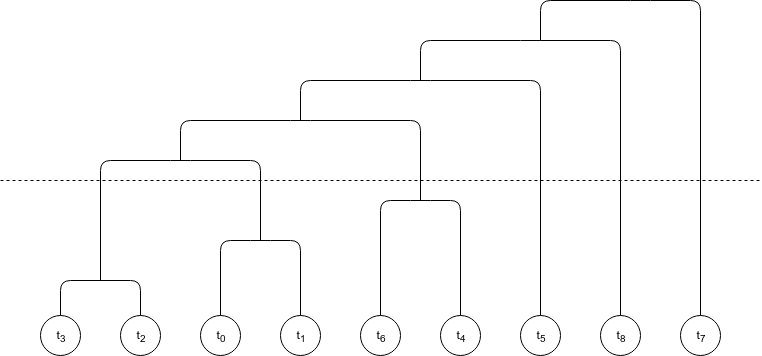
\includegraphics[width=\textwidth]{img/CF.png}
    \caption{The horizontal line represents a cut of the dendrogram
    and defines the coalition structure.}
    \label{fig:CF_graph}
\end{figure}

The result of the Set Partition is:

  \begin{center}
    \begin{tabular}{|c|c|c|c|} \hline
    \textbf{task} & \textbf{item} & \textbf{demand} & \textbf{unloading bay} \\ \hline
    \{4,7\}    & B    & 4     & \{1\}             \\
    \{0,1,3\}  & \{A,B\}& 4    & \{0,1\}             \\
    \{2,6\}    & \{C,A\}    & 4  & \{0,2\}             \\
    5    & C    & 3      & 2             \\
    8    & C    & 3      & 2             \\ \hline       
    \end{tabular}
  \end{center}
